\section{\\Parâmetros do sistema de suspensão ativa}
\begin{table}[h!]
\centering
    \begin{tabular}{|c|c|c|}
        \hline
        Parâmetro & Valor & Unidade\\
        \hline
        \hline
        $m_s$& $290$& $kg$\\
        $m_u$& $40$& $kg$\\
        $b^{l}_s$& $700$& $Ns.m^{-1}$\\
        $b^{nl}_s$& $200$& $Ns.m^{-1}$\\
        $b^{y}_s$& $400$& $Ns.m^{-1}$\\
        $k^{l}_s$& $235.10^2$& $N.m^{-1}$\\
        $k^{nl}_s$& $235.10^4$& $N.m^{-1}$\\
        $k_t$& $190.10^3$& $N.m^{-1}$\\
        \hline
    \end{tabular}    \label{tb:parametros}\caption{Parâmetros da suspensão ativa não linear, fonte \cite{MarceloTusset2008MINISTERIOPor}.}
\end{table}
\section{\\Lista de siglas e abreviações}
    \begin{itemize} 
        \item [LTI] Linear e invariante no tempo.
        \item [UIO] Observador de entradas desconhecidas.
        \item [SISO] Single Input, Single Output.
        \item [LMI] Desigualdade Matricial Linear.
        \item [LPV] Sistemas lineares com dependência paramétrica.
        %\item [$m_s$] Massa suspensa.
%        \item [$m_u$] Massa não suspensa.
 %       \item [$b_s$] Coeficiente de amortecimento do amortecedor passivo. 
   %     \item [$k_s$] Coeficiente de elasticidade do feixe de molas da suspensão.
   %     \item [$k_t$] Coeficiente de elasticidade do pneu.
     %   \item [$x_r$] Deslocamento vertical da pista.
 %       \item [$x_w$] Deslocamento vertical da roda.
 %       \item [$x_c$] Deslocamento vertical da carroceria.
     %   \item [$\dot{x}_w$] Velocidade vertical da roda.
  %      \item [$\dot{x}_c$] Velocidade vertical da carroceria.
  %      \item [$F$] Força aplicada pelo amortecedor ativo ou semi-ativo.
 %       \item [$k^{l}_{s}$] Coeficiente de elasticidade do termo linear no modelo %não linear do feixe de olas da suspensão.
 %       \item [$k^{nl}_{s}$] Coeficiente de elasticidade do termo não linear no %modelo não linear do feixe de molas da suspensão.
 %       \item [$b^{l}_{s}$] Coeficiente de amortecimento do termo da faixa de %operação linear do amortecedor.
  %     \item [$b^{l}_{s}$] Coeficiente de amortecimento do termo da faixa de %operação não linear do amortecedor.
   %     \item [$b^{y}_{s}$] Coeficiente que representa a característica  de %comportamento assimétrico do amortecedor.
    \end{itemize}
%\section{}\listoffigures
\FloatBarrier
\section{\\Experimentos em simulink}
\begin{figure*}
    \centering
    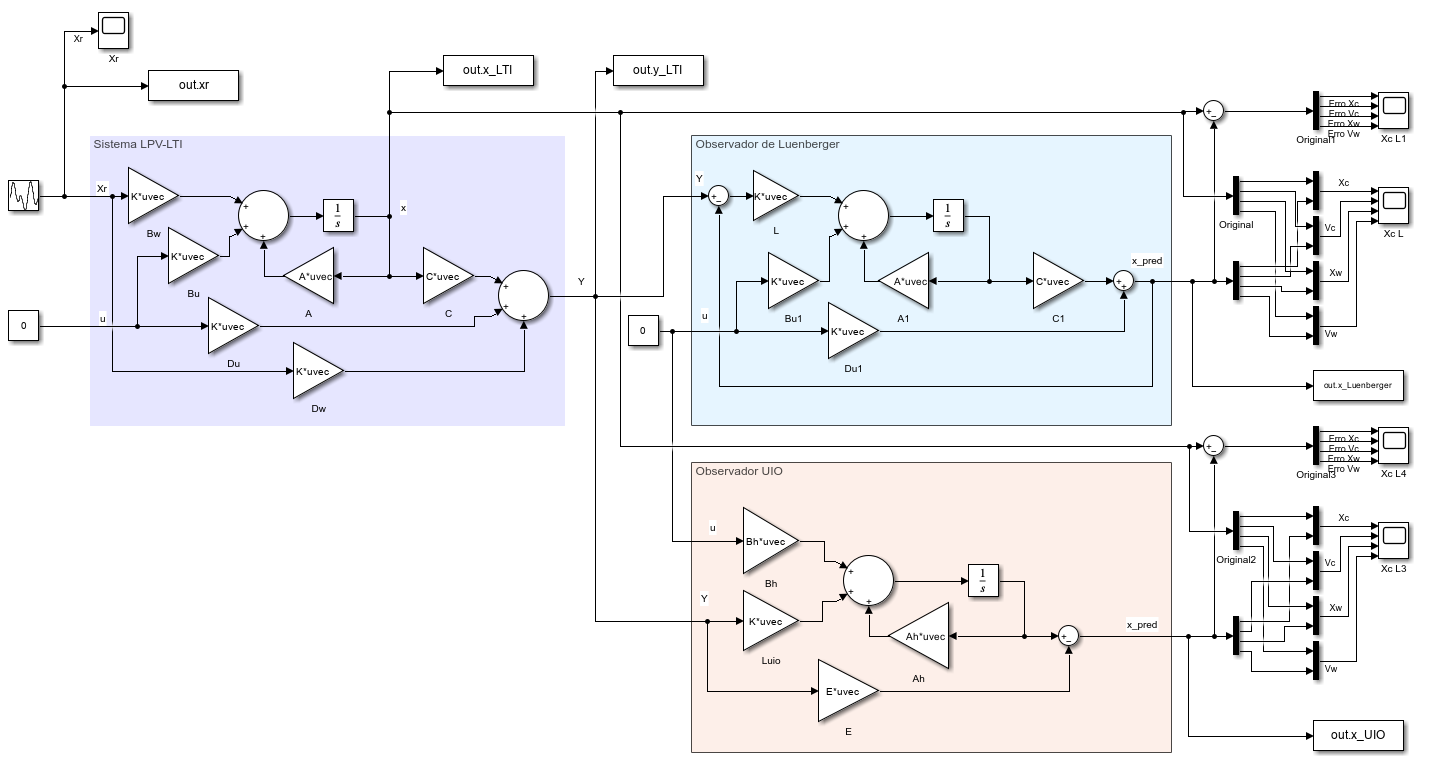
\includegraphics[width=0.8\textwidth]{img/setup_teste_observador.png}
    \caption{Experimento em simulink para teste dos observadores Luenberger e UIO.}
    \label{fig:setup_testeobs}
\end{figure*}
\begin{figure*}
    \centering
    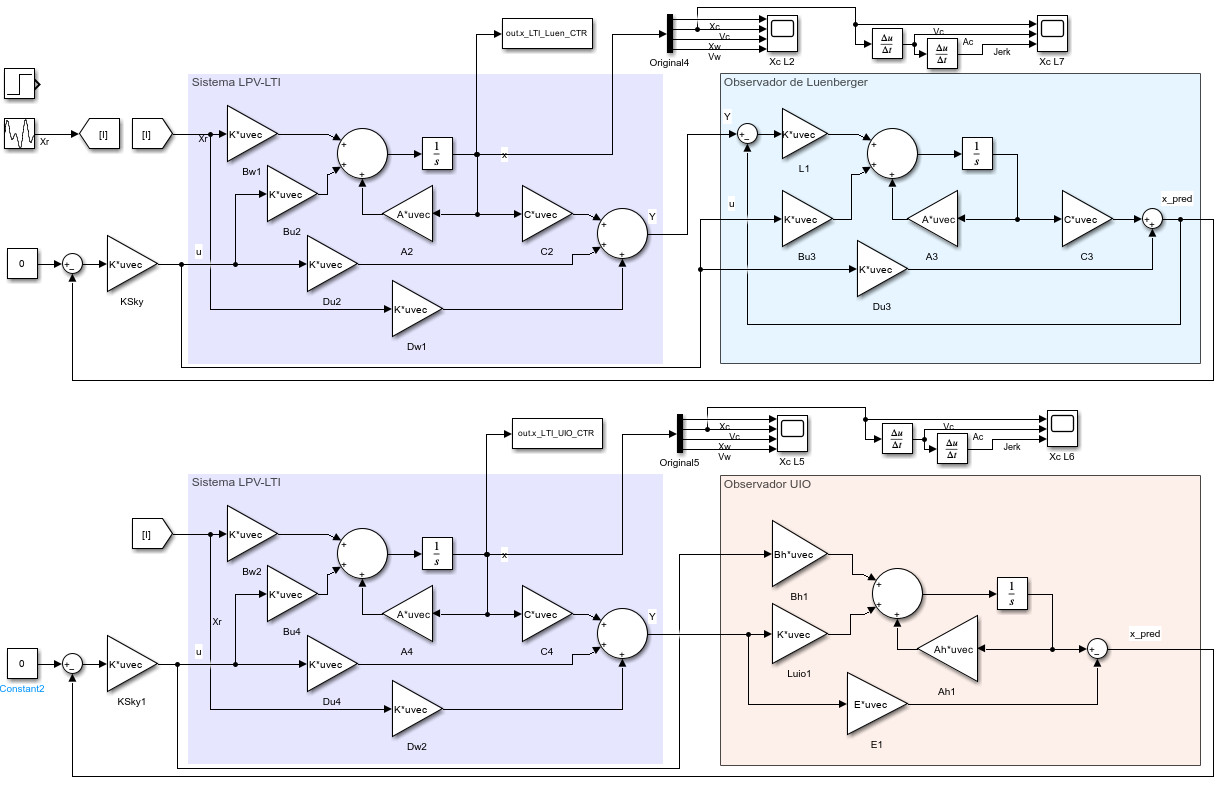
\includegraphics[width=0.8\textwidth]{img/setup_teste_controlador.png}
    \caption{Experimento em simulink para teste do desempenho das extratégis de controle empregando observadores de Luenberger e UIO.}
    \label{fig:setup_testectr}
\end{figure*}
\FloatBarrier
